\documentclass[a4paper, 12pt]{article}
\usepackage[spanish]{babel}
\usepackage[utf8]{inputenc}
\usepackage{amsmath}
\usepackage{indentfirst}
\usepackage{graphicx}
\usepackage[colorinlistoftodos]{todonotes}
\usepackage{esint}
\usepackage{multicol}
\usepackage{listings}
\usepackage{xcolor}

\usepackage[a4paper,
            bindingoffset=0.2in,
            left=2.5cm,
            right=2.5cm,
            top=2.5cm,
            bottom=2.5cm,
            footskip=30pt]{geometry}

\definecolor{codegreen}{rgb}{0,0.6,0}
\definecolor{codegray}{rgb}{0.5,0.5,0.5}
\definecolor{codepurple}{rgb}{0.58,0,0.82}
\definecolor{backcolour}{rgb}{0.95,0.95,0.92}

\lstdefinestyle{customc}{
	language=C,
    backgroundcolor=\color{backcolour},   
    commentstyle=\color{codegreen},
    keywordstyle=\color{magenta},
    numberstyle=\tiny\color{codegray},
    stringstyle=\color{codepurple},
    basicstyle=\ttfamily\footnotesize,
    breakatwhitespace=false,         
    breaklines=true,                 
    captionpos=b,                    
    keepspaces=true,                 
    numbers=left,                    
    numbersep=5pt,                  
    showspaces=false,                
    showstringspaces=false,
    showtabs=false,                  
    tabsize=2
}

\lstdefinestyle{customasm}{
	language=[x86masm]Assembler,
    backgroundcolor=\color{backcolour},   
    commentstyle=\color{codegreen},
    keywordstyle=\color{magenta},
    numberstyle=\tiny\color{codegray},
    stringstyle=\color{codepurple},
    basicstyle=\ttfamily\footnotesize,
    breakatwhitespace=false,         
    breaklines=true,                 
    captionpos=b,                    
    keepspaces=true,                 
    numbers=left,                    
    numbersep=5pt,                  
    showspaces=false,                
    showstringspaces=false,
    showtabs=false,                  
    tabsize=2
}

\lstset{escapechar=@,style=customasm}

\lstset{literate=
  {á}{{\'a}}1 {é}{{\'e}}1 {í}{{\'i}}1 {ó}{{\'o}}1 {ú}{{\'u}}1
  {Á}{{\'A}}1 {É}{{\'E}}1 {Í}{{\'I}}1 {Ó}{{\'O}}1 {Ú}{{\'U}}1
  {à}{{\`a}}1 {è}{{\`e}}1 {ì}{{\`i}}1 {ò}{{\`o}}1 {ù}{{\`u}}1
  {À}{{\`A}}1 {È}{{\'E}}1 {Ì}{{\`I}}1 {Ò}{{\`O}}1 {Ù}{{\`U}}1
  {ä}{{\"a}}1 {ë}{{\"e}}1 {ï}{{\"i}}1 {ö}{{\"o}}1 {ü}{{\"u}}1
  {Ä}{{\"A}}1 {Ë}{{\"E}}1 {Ï}{{\"I}}1 {Ö}{{\"O}}1 {Ü}{{\"U}}1
  {â}{{\^a}}1 {ê}{{\^e}}1 {î}{{\^i}}1 {ô}{{\^o}}1 {û}{{\^u}}1
  {Â}{{\^A}}1 {Ê}{{\^E}}1 {Î}{{\^I}}1 {Ô}{{\^O}}1 {Û}{{\^U}}1
  {ã}{{\~a}}1 {ẽ}{{\~e}}1 {ĩ}{{\~i}}1 {õ}{{\~o}}1 {ũ}{{\~u}}1
  {Ã}{{\~A}}1 {Ẽ}{{\~E}}1 {Ĩ}{{\~I}}1 {Õ}{{\~O}}1 {Ũ}{{\~U}}1
  {œ}{{\oe}}1 {Œ}{{\OE}}1 {æ}{{\ae}}1 {Æ}{{\AE}}1 {ß}{{\ss}}1
  {ű}{{\H{u}}}1 {Ű}{{\H{U}}}1 {ő}{{\H{o}}}1 {Ő}{{\H{O}}}1
  {ç}{{\c c}}1 {Ç}{{\c C}}1 {ø}{{\o}}1 {å}{{\r a}}1 {Å}{{\r A}}1
  {€}{{\euro}}1 {£}{{\pounds}}1 {«}{{\guillemotleft}}1
  {»}{{\guillemotright}}1 {ñ}{{\~n}}1 {Ñ}{{\~N}}1 {¿}{{?`}}1 {¡}{{!`}}1  {°}{{$^\circ$}}1
}

\setlength{\marginparwidth}{2cm}
\begin{document}
\begin{titlepage}
	\begin{center}
		{\large{UNIVERSIDAD TECNOLÓGICA NACIONAL}}
	\end{center}
	\vspace{15pt}
	\begin{figure}[!ht]
		\centering
		\begin{center}
			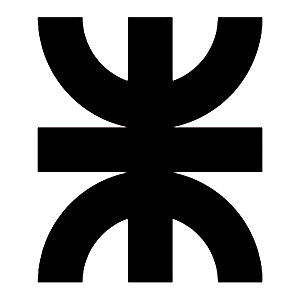
\includegraphics[width=5cm]{utn.png}
		\end{center}
	\end{figure}
	\vspace{5pt}
	\begin{center}
		{\large{FACULTAD REGIONAL PARANÁ}}
		\vspace{5pt}
		\begin{center}
			\vspace{15pt}
			\normalsize{CARRERA: Ingeniería Electrónica\\
						CÁTEDRA: Técnicas Digitales II\\}
			\vspace{50pt}
			\huge\bfseries{Trabajo Práctico N°10\\
			Control de intensidad de LED con PWM\\}
			\vspace{50pt}
		\end{center}
		
		\begin{flushleft}
			\begin{center}
				ALUMNOS:\\
				Battaglia Carlo\\
				Escobar Gabriel\\
			\end{center}
		\end{flushleft}
		
		\begin{center}
			\vspace{\fill}
			\normalsize{Paraná,}
			\today
		\end{center}
	\end{center}
\end{titlepage}

\newpage
\pagenumbering{arabic}
\numberwithin{equation}{section}

\section{Actividades}

\textbf{1.} El circuito “base” del cual se deberá partir es el utilizado en el trabajo práctico Nro 8.

\textbf{2.} El circuito deberá tener, además:

\quad	\textbf{a.} Un teclado matricial de 3x3 teclas, dispuestos convenientemente.

\textbf{3.} El funcionamiento general del circuito es:

\quad	\textbf{a.} El sistema, al encendido, deberá estar todo apagado (incluido el display).

\quad	\textbf{b.} En la medida que se presiona una tecla, se deberá mostrar la tecla presionada en el display (de 1 a 9).

\quad	\textbf{c.} Transcurridos 3 segundos, y si no se presiona ninguna tecla, se apagará el display que indica la tecla presionada.

\quad	\textbf{d.} En el momento que se presiona la tecla, se enviará una cadena hacia la computadora informando la tecla presionada. Dicha cadena será:

\qquad	\textbf{i.} \$TD2,$<$número tecla$>$*

\qquad \textbf{ii.} Donde $<$número tecla$>$ es el valor ASCII de la tecla presionada. Los símbolos $<$ y $>$ no se envían.
	
\qquad \textbf{iii.} Ejemplo: Se presiona la tecla número 3, se envía a la PC la cadena \$TD2,3*

\section{Código}

En el primer bloque de código hacemos las declaraciones correspondientes. 

Renombramos los registros $r16$ y $r17$ como $temp$ y $aux$.

Declaramos al registro general de entrada/salida $GPIOR0$ para utilizarlo a modo de registro de banderas, en el que alojaremos la bandera $PressKey$ para detectar pulsaciones del teclado, y $ContarSeg$ para contar segundos.
\begin{lstlisting}
;
;************************************
; Técnicas Digitales II 
; Autor: Battaglia - Escobar
; for AVR: atmega328p (Arduino UNO)
; clock frequency: 16MHz 
;************************************

.ifndef F_CPU
.set F_CPU = 16000000
.endif
;===========================================
; Declarations for register
.def temp 		= r16
.def aux		= r17

;===========================================
; Declarations for label
.set Flags0			= GPIOR0
.set PressKey		= $0
.set ContarSeg		= 1

;===========================================
; Etiquetas
.equ	baud = 9600			;Baud Rate

;===========================================
; Data Segment
.dseg
DATA_KB:			.byte	1
tres_seg:			.byte	1
BaseTime1ms:		.byte	1
BaseTime20ms:		.byte	1
BaseTime100ms:		.byte	1

;===========================================
; EEPROM Segment
.eseg
VAR_EEPROM:		.db		$AA

;===========================================
; Code Segment
.cseg
.org RWW_START_ADDR 
\end{lstlisting}

Seguidamente, en el cuerpo principal del programa, inicializamos la el $Stack Pointer$ apuntándolo a la parte baja de la memoria RAM.

Luego llamamos a las funciones correspondientes para inicializar la USART0, el TIMER0 y los puertos. Cada una de estas funciones será abordada más adelante.

Antes de entrar en el bucle principal, habilitamos las interrupciones.

Ahora sí en el bucle principal $loop$, esperamos hasta que la bandera $PressKey$ indique la pulsación de una tecla, enviando entonces el código ``$\$TD2,-*\setminus n$'', con el número presionado en lugar del $-$.

Luego se baja la bandera en cuestión y se escribe el digito en $PORTD$.

Finalmente levantamos la bandera $ContarSeg$, para indicar que debe comenzar a contarse 3 segundos antes de apagar el display nuevamente.

\begin{lstlisting}
;======================
; Main body of program:
Reset:
	ldi R16, LOW(RAMEND)    	; Lower address byte RAM byte lo.
	out SPL, R16         		; Stack pointer initialise lo.
	ldi R16, HIGH(RAMEND)   	; Higher address of the RAM byte hi.
	out SPH, R16			 	; Stack pointer initialise hi. 
; write your code here
	call Init_USART0
	call Init_Timer0
	call Init_Port
			
	;ldi r19,(1 << DDB5)
	;out DDRB, r19

	;clr r18
	sei
Loop:
	;sbic Flags0, TresSeg
	;rcall display_off

	sbis Flags0,PressKey				 
	rjmp Loop

	ldi temp, '$'
	rcall Tx_Byte_USART0		; Send Byte
	ldi temp, 'T'
	rcall Tx_Byte_USART0		; Send Byte
	ldi temp, 'D'
	rcall Tx_Byte_USART0		; Send Byte
	ldi temp, '2'
	rcall Tx_Byte_USART0		; Send Byte
	ldi temp, ','
	rcall Tx_Byte_USART0		; Send Byte
	lds	temp,DATA_KB
	rcall Tx_Byte_USART0		; Send Byte
	ldi temp, '*'
	rcall Tx_Byte_USART0		; Send Byte
	ldi temp, '\n'
	rcall Tx_Byte_USART0		; Send Byte

	in temp, Flags0						; Tecla enviada
	cbr temp, (1 << PressKey)			; PressKey = 0 en Flags0
	out Flags0, temp

	rcall write_digit

	clr temp
	sts tres_seg, temp			;reseteo el contador de 3 segundos

	in temp, Flags0
	sbr temp, (1 << ContarSeg)	;empiezo a contar 3 segundos
	out Flags0, temp

	rjmp Loop            ; loop back to the start

\end{lstlisting}

Esta subrutina inicializa el timer 0 en modo normal con un preescalado de 64 y habilita las interrupciones por overflow.

\begin{lstlisting}
;===========================================
; Init_Timer0
; Inicia el Timer 0 para desborde cada 1 mseg
; Tovf = 2^n * Prescaler / Fio
; Mod = Tovf * Fio / Prescaler
Init_Timer0:
	;Set the Timer Mode to Normal
	;TCCR0A
	; COM0A1 | COM0A0 | COM0B1 | COM0B0 | - | - | WGM01 | WGM00
	;	0		 0		  0		   0				0		0
	in	temp,TCCR0A
	cbr	temp,1<<WGM00
	cbr	temp,1<<WGM01
	out TCCR0A,temp
	
	;TCCR0B
	; FOC0A	| FOC0B | - | - | WGM02 | CS02 | CS01 | CS00
	;	0		0				0		0	   1	  1
	in	temp,TCCR0B
	cbr	temp,1<<WGM02
	out TCCR0B,temp
	
	;Activate interrupt for Overflow
	;TIMSK0
	; -	| - | - | - | - | OCIE0B | OCIE0A | TOIE0
	;						0		 0		  1
	lds	temp,TIMSK0
	sbr	temp,1 << TOIE0
	sts TIMSK0,temp
	
	;Set TCNT0
	ldi	temp,6
	out TCNT0,temp
	
	;Start the Timer (prescaler %64)
	in	temp,TCCR0B
	sbr	temp,1<<CS00
	sbr	temp,1<<CS01
	cbr	temp,1<<CS02
	out TCCR0B,temp
	ret
\end{lstlisting}

\textit{Init\_Port} inicializa los puertos a utilizar, poniendo a los puertos D y C como salida y al puerto B como entrada.

\begin{lstlisting} 
;===========================================
; Init_Port
; Inicia el Puerto PD7-4 como salida
; Puerto C3-C0 como entrada
Init_Port:
	ldi temp, (1<<DDD7) | (1<<DDD6) | (1<<DDD5) | (1<<DDD4)
	out DDRD, temp			; PortD como salida
	clr temp				; Borro el PortD
	ldi temp, (1<<PD7) | (1<<PD6) | (1<<PD5) | (0<<PD4)
	out PORTD, temp			;Puerto en ALTO

	ldi temp, (1<<DDC5) | (1<<DDC4) | (1<<DDC3) | (1<<DDC2) | (1<<DDC1) | (1<<DDC0)
	out DDRC, temp			; PortC como salida
	clr temp				; Borro el PortC
	out PORTC, temp
	
	ldi aux, (1<<DDB3) | (1<<DDB2) | (1<<DDB1) | (1<<DDB0)
	out PORTB, aux			; Activo resistencias de Pull-Up
	out DDRB, temp			; PortB como entrada

	ret
\end{lstlisting}	  

La subrutina \textit{Init\_USART0} inicializa la transmisión serie a una velocidad de 9600 baudios.

\begin{lstlisting}
;===========================================
; Init_USART0
; Inicializa la transmisión serie: 8N1 9600
; Parámetro: No
; Retorno: No
Init_USART0:
{
			;Set Baud Rate
			ldi	r17,high(F_CPU/(16*baud)-1)	
			ldi	r16,low(F_CPU/(16*baud)-1)	
			sts UBRR0H, r17
			sts UBRR0L, r16
			
			; Enable receiver and transmitter
			ldi r16, (1<<TXEN0)		
			sts UCSR0B,r16

			; Set frame format: 8data, 1stop bit
			ldi r16, (0<<USBS0)|(3<<UCSZ00)		
			sts UCSR0C,r16
			ret
}
\end{lstlisting}

Y \textit{Tx\_Byte\_USART0} envía bytes individuales a través de la comunicación serie ya establecida.

\begin{lstlisting}
;===========================================
; Tx_Byte_USART0
; Envía dato por USART0
; Parámetro: R16 -> dato que se envía
; Retorno: No
Tx_Byte_USART0:
{
		   ; Wait for empty transmit buffer
		   lds r17,UCSR0A			;Load into R17 from SRAM UCSR0A         
		   sbrs r17,UDRE0			;Skip next instruction If Bit Register is set
		   rjmp Tx_Byte_USART0
		   ; Put data (r16) into buffer, sends the data
		   sts UDR0,r16
		   ret
}
\end{lstlisting}

En cuanto a las interrupciones, hacemos uso de la interrupción por overflow del $timer0$.

Como previamente definimos un preescalado de 64, y la frecuencia de trabajo del microcontrolador es $16[MHz]$, la frecuencia resultante es $250[kHz]$.

Dado que timer 0 es de 8 bits, sabemos que ocurrirá una interrupción por overflow cada $255*1/250000[s]$, es decir, $1.02[ms]$.

Si en lugar de contar desde 0 forzamos al timer a contar a partir de 6, la interrupción ocurrirá cada 250 pulsos de clock. Esto se traduce entonces a $250*1/250000[s]$, lo que equivale exactamente a $1[ms]$.

Esto nos permite contar milisegundos de forma directa, y lo utilizaremos para esperar $200[ms]$ entre cada lectura de teclado.

A su vez, utilizaremos esta cuenta de $200[ms]$ para detectar el paso de $3[s]$. Esto lo logramos contando 15 veces la ocurrencia de los 200 overflows anteriores, esto es $15*200[ms]=3000[ms]=3[s]$, y utilizaremos esta referencia temporal para apagar el display.

\begin{lstlisting}
;==========================
; Rutinas de interrupción

isr_OVF0_handler:
	push temp
	ldi	temp,6
	out TCNT0,temp
	lds temp, BaseTime1ms
	inc temp
	cpi temp,200			;chequea si pasaron 200ms
	brne notime
	rcall Read_KEY			;Leo el teclado
	ldi temp, 0
	sbis Flags0, ContarSeg
	rjmp notime
	lds temp, tres_seg
	inc temp
	cpi temp, 15			;si pasaron 15 veces 200ms son 3000ms=3s
	brne no_3_seg
	
	rcall display_off

	ldi temp, 0
no_3_seg:
	sts tres_seg, temp
	ldi temp, 0
notime:
	sts BaseTime1ms, temp
	pop temp
	reti					; Timer0 overflow interrupt  
\end{lstlisting}

La siguiente subrutina \textit{Read\_KEY} lee la tecla presionada en el teclado matricial y la escribe directamente sobre $PORTD$, donde se encuentra conectado el display de 7 segmentos.

\begin{lstlisting}
;===========================================
; Read_KEY
; Lee un teclado matricial y escribe directamente a PORTD
; Parámetro: No 
Read_KEY:
ROW_1:
	;ldi aux,0x70	;Activo R1		0111 0000
	;out PORTD,aux
	CBI	PORTD,7
	nop
	in	temp,PINB
	andi temp,0x0f
	cpi	temp,0x0b	;0000 1011
	breq IS_KEY_3
	cpi	temp,0x0d	;0000 1101
	breq IS_KEY_2
	cpi	temp,0x0e	;0000 1110
	breq IS_KEY_1
	rjmp ROW_2
IS_KEY_3:
	ldi	temp,'3'
	sts	DATA_KB,temp
	in temp, Flags0					; Tecla presionada
	sbr temp, (1 << PressKey)		; PressKey = 1 en Flags0
	out Flags0, temp
	rjmp out_read_key
IS_KEY_2:
	ldi	temp,'2'
	sts	DATA_KB,temp
	in temp, Flags0					; Tecla presionada
	sbr temp, (1 << PressKey)		; PressKey = 1 en Flags0
	out Flags0, temp
	rjmp out_read_key
IS_KEY_1:
	ldi	temp,'1'
	sts	DATA_KB,temp
	in temp, Flags0					; Tecla presionada
	sbr temp, (1 << PressKey)		; PressKey = 1 en Flags0
	out Flags0, temp
	rjmp out_read_key
ROW_2:
	;ldi aux,0xB0	;Activo R2		1011 0000
	;out PORTD,aux
	SBI	PORTD,7
	CBI	PORTD,6
	nop
	in	temp,PINB
	andi temp,0x0f
	cpi	temp,0x0b	;0000 1011
	breq IS_KEY_6
	cpi	temp,0x0d	;0000 1101
	breq IS_KEY_5
	cpi	temp,0x0e	;0000 1110
	breq IS_KEY_4
	rjmp ROW_3
IS_KEY_6:
	ldi	temp,'6'
	sts	DATA_KB,temp
	in temp, Flags0					; Tecla presionada
	sbr temp, (1 << PressKey)		; PressKey = 1 en Flags0
	out Flags0, temp
	rjmp out_read_key
IS_KEY_5:
	ldi	temp,'5'
	sts	DATA_KB,temp
	in temp, Flags0					; Tecla presionada
	sbr temp, (1 << PressKey)		; PressKey = 1 en Flags0
	out Flags0, temp
	rjmp out_read_key
IS_KEY_4:
	ldi	temp,'4'
	sts	DATA_KB,temp
	in temp, Flags0					; Tecla presionada
	sbr temp, (1 << PressKey)		; PressKey = 1 en Flags0
	out Flags0, temp
	rjmp out_read_key
ROW_3:
	;ldi aux,0xD0	;Activo R3		1101 0000
	;out PORTD,aux
	SBI	PORTD,6
	CBI	PORTD,5
	nop
	in	temp,PINB
	andi temp,0x0f
	cpi	temp,0x0b	;0000 1011
	breq IS_KEY_9
	cpi	temp,0x0d	;0000 1101
	breq IS_KEY_8
	cpi	temp,0x0e	;0000 1110
	breq IS_KEY_7
	rjmp out_read_key
IS_KEY_9:
	ldi	temp,'9'
	sts	DATA_KB,temp
	in temp, Flags0					; Tecla presionada
	sbr temp, (1 << PressKey)		; PressKey = 1 en Flags0
	out Flags0, temp
	rjmp out_read_key
IS_KEY_8:
	ldi	temp,'8'
	sts	DATA_KB,temp
	in temp, Flags0					; Tecla presionada
	sbr temp, (1 << PressKey)		; PressKey = 1 en Flags0
	out Flags0, temp
	rjmp out_read_key
IS_KEY_7:
	ldi	temp,'7'
	sts	DATA_KB,temp
	in temp, Flags0					; Tecla presionada
	sbr temp, (1 << PressKey)		; PressKey = 1 en Flags0
	out Flags0, temp
	;rjmp out_read_key
out_read_key:
	in aux, PORTD
	ori aux,0xE0					;Desactivo los renglones
	out PORTD,aux
	ret 
\end{lstlisting}

La subrutina encargada de apagar el display es la siguiente, \textit{display\_off}. Ésta apaga todos los segmentos del display y resetea la bandera $ContarSeg$, puesto que ya pasaron 3 segundos.

\begin{lstlisting}
display_off:
	clr temp
	out PORTC, temp
	cbi PORTD, 4

	in temp, Flags0
	cbr temp, (1 << ContarSeg)	;dejo de contar 3 segundos
	out Flags0, temp

	ret
\end{lstlisting}

La siguiente subrutina convierte el dígito almacenado en \textit{DATA\_KB} a 7 segmentos y lo muestra en el display conectado a $PORTD$.

\begin{lstlisting}
write_digit:
	push temp
	lds temp, DATA_KB
	subi temp, 0x30
	rcall BCD_to_7_segment
	out PORTC, r16
	cbi PORTD, 4
	sbrc temp, 6
	sbi PORTD, 4
	pop temp
ret
\end{lstlisting}

La función que convierte los números BCD a su codificación en 7 segmentos es la siguiente, que hace uso de una tabla de conversión.

\begin{lstlisting}
;===========================================
; BCDTo7Segment
;
; Convierte el valor, pasado en el registro r16, a una representación en 
; display de 7 segmentos, de manera que:
; Dp g f e d c b a
; B7 B6 B5 B4 B3 B2 B1 B0
;
BCD_to_7_segment:
push ZH
push ZL
ldi ZH,HIGH(2*BCDTo7Seg) ; Carga la tabla
ldi ZL,LOW(2*BCDTo7Seg)
add ZL,r16
lpm
mov r16,R0
pop ZL
pop ZH
ret

; Tabla de conversión decimal a 7 segmentos
BCDTo7Seg:
.db 0x3F,0x06,0x5B,0x4F,0x66,0x6D,0x7D,0x07,0x7F,0x6F
\end{lstlisting}


 
\end{document}
